\begin{usecase}{Continue with Email}
  \ucbasicinfo{High}{Regular}
  \ucshortdescription{This UC allows users to login or create an account using their email.}
  \uctrigger{This UC starts when the user enters their email to the system.}
  \ucactors{User}{None}
  \ucpreconditions{User must have an email}
  \ucrelationships{Send Welcome Email}{N/A}{N/A}
  \ucinputsoutputs{
    \begin{itemize}
      \item \textbf{Email} (Source: User)
      \item \textbf{Magic Link (from email)} (Source: User)
    \end{itemize}
  }{
    \begin{itemize}
      \item \textbf{Magic link email} (Destination: User)
      \item \textbf{Confirmation messages} (Destination: User Interface)
      \item \textbf{JWT} (Destination: App)
    \end{itemize}
  }
  \ucmainflow{
    \begin{enumerate}
      \item The user enters their email.
            \ucinfo{System displays an email input field.}
      \item System creates an account if the user has no account, and then generates and sends the magic link.
            \ucinfo{App displays ``Check your email'' message.}
      \item The user clicks the magic link in the email.
            \ucinfo{The app is opened on the device of the user.}
      \item The app sends the token to the system to log the user in.
            \ucinfo{System verifies token and logs user in.}
    \end{enumerate}
  }
  \ucalternateflows{
    \begin{itemize}
      \item The user cancels the authentication request.
    \end{itemize}
  }
  \ucexceptions{
    \begin{itemize}
      \item Invalid email format.
      \item Magic link token expired or invalid.
      \item \textbf{Request sending failure}: If sending the request fails due to network issues, the system prompts the user to try again.
    \end{itemize}
  }
  \ucconclusion{This UC ends when the user is logged in.}
  \ucpostconditions{The system generates a JWT.}
  \ucspecialrequirements{An email server must be present to send magic link email.}
\end{usecase}

\begin{figure}[!h]
  \centering
  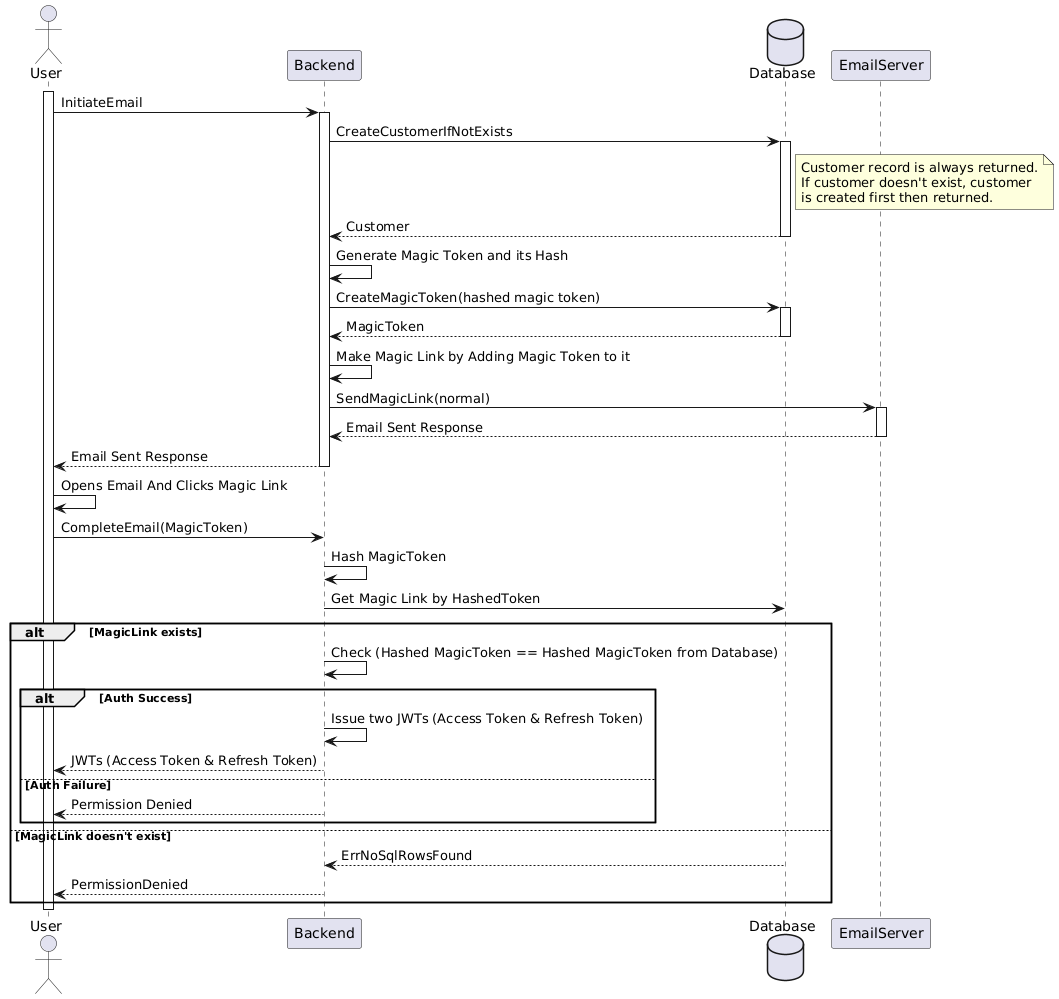
\includegraphics[width=\textwidth]{images/docs/diagrams/sequence-diagrams/all-sequence-diagrams/Continue with Email.png}
  \caption{Continue with Email Sequence Diagram}
  \label{fig:seq/continue-with-email}
\end{figure}

The "Continue with Email Sequence Diagram", shown in \textbf{Figure~\ref{fig:seq/continue-with-email}}, illustrates the process of email-based magic link authentication, involving interactions between the User, Backend, Database, and EmailServer. The process begins when the user initiates email authentication process. The backend executes the CreateCustomerIfNotExists function to retrieve an existing customer record or create a new one if none exists. Once the customer is identified, the backend generates a magic token and its hashed version using the GenerateMagicToken function. The hashed token is stored in the database, and a magic link containing the token is created. The backend then sends the magic link to the user's email using the SendEmail function via the email server. The user clicks the magic link, triggering the CompleteFlow(MagicToken) request to the backend, where the provided token is validated against the stored hashed token in the database. If the tokens match, authentication succeeds, and the backend issues a JSON Web Token (JWT) to the user for future access. In cases where the token is invalid, expired, or the customer record is missing, the system responds with appropriate errors, such as PermissionDenied or EntryNotFound. This diagram demonstrates a secure flow for handling authentication via email magic links.